\documentclass[a4paper, 12pt]{article}


\usepackage{graphicx}
\usepackage{xcolor}
\usepackage{mdframed}
\usepackage { amsmath , amssymb , amsthm }
\usepackage[T2A]{fontenc}
\usepackage[utf8]{inputenc}
\usepackage[english,russian]{babel}

\graphicspath{{img/}}
\DeclareGraphicsExtensions{.pdf,.png,.jpg}


\title{Математический анализ}
\author{Алла Владимировавна Устюжанова}
\date{\today}

\begin{document}
\sffamily
\maketitle
\section*{Лекция 1}

\section{Глава 1. Введение. }
\subsection{Параграф 1: Множества операции над множествами}
Кванторы:
\[
	\forall \quad \exists
\]
Множество -- это совокупность каких-либо предметов(элементов).
\[
	A \quad B , \\\quad
	x \in A,\\ \quad
	x \not\in B,	\\\quad
	A \in B\\
\]
Операции: \\
1. $ A \cup B $ -- те множество каждый элемент которого принадлежит хотябы одному из множеств A или B \[
	A \cup B = \{x:x \in A \quad or \quad x \in B\}	
\]
2. $ A \cap B $ -- это множество каждый элемент которого принадлежит одновременне и A и B \[
	 A \cap B = \{x: x\in A \quad and \quad x \in B\}	
\]
3. $ A \setminus B $ -- (Разность)\[
	A \setminus B = \{x: x\in A \quad but \quad x\not\in B\}	
\]
4. $ CA \quad\bar{A} $ -- (Дополнение) \[
	CA = \bar{A} - S\setminus A	
\]


Виды множеств:\\
$ N \subset Z \subset Q \subset R \subset C $\\

\subsection{Абсолютная величина}
\[
	|x| = \{x \quad x \geq 0 \quad or \quad -x \quad x\leq 0\}	
\]
\subsubsection*{Свойства:}
1. Неравенство треугольника \[
 |x+y| = |x| + |y|	
\]
\begin{mdframed}[backgroundcolor=blue!20] 
       Док-во: пусть $  x+y \geq 0\Rightarrow |x+y| = x+y=|x|+|y|$\\
       Док-во: пусть $  x+y < 0\Rightarrow |x+y| = x+(-y)<|x|+|y|$
    \end{mdframed}

2. $  |x - y|= |x| - |y|$ если $ |x| > |y| $
3. $ |xyz| = |x||y||z| $
4. $ \left| \frac{x}{y}\right| =  \frac{|x|}{|y|}$
sgn x = $ \{ 1 \quad x>0 \quad 0 \quad x=0\} $\\

\subsubsection*{Бином Ньютона:}
\[
	\left( a + b\right)^n = a^n + C_n^1 a^{n-1}b +...+b^n	
\]
\[
	C_n^k = \frac{n!}{(n-k)!k!}	
\]

\[
	n! = 1\cdot 2 \cdot 3 \cdot ... \cdot n	
\]
\[
	0! = 1	
\]


\subsubsection*{Треугольник Паскаля:}
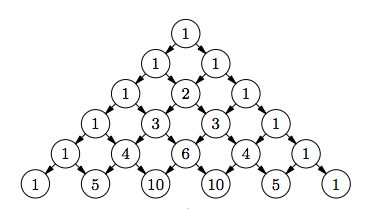
\includegraphics{Pascal_triangle}

\subsubsection{Упражнения}
1. $ A=\{1,2,3\} \quad B=\{2,3,4,5\} \quad A\cup B ? $\\
2. $ A = \{x \in N: \quad 2 < x < 4\} \quad B = \{x \in N: \quad 2 < x < 4\} \quad C = \{x \in N: \quad 2 < x < 4\} \quad B\cup C ?, A\cap B\cap C,A\cup B\cup C \quad ?$\\
3. $ (A\cap B)\cup C = (A\cup C)\cap(B\cup C)? $\\
4. $ (A \setminus B)\cap C = (A\cap C)\setminus (B\cap C) $\\
5. $ \left( 1-x\right)^5 = ?\\$
6. $ \left(\frac{2}{x} + 3 \sqrt[]{x} \right)^4 $\\
\section{Глава 2. Предел и непрерывность.}
\begin{mdframed}[backgroundcolor=blue!20] 
       Курс: Мат анализ (фтф:ИВТ)\\
       код слово: предел
    \end{mdframed}
\subsection{Параграф 1. Предел псоледовательности}
Предел -- пусть каждому натуральному числу N по некоторому закону поставленно в соответствие действительное число $ x_n $ тогда говорят что определена числовая последовательность $ \{x\} = \{x_1,x_2,....,x_n,...\} $ \\
Число a называется пределом последовательности $ \{x_n\}  $ если для всякого действительного числа $ \epsilon  > 0$ найдется зависящее от $ \epsilon $ число такое что выполняется неравенство $ |x_n - a| < \epsilon  $ для всех натуральных чисел $ n > n_0 $.  \\
\\Обозначение:\\
\[
	\lim_{n\to 0} x_n  = a \quad(x_n \to a \quad n \to \inf)	
\]
 
 \[
 	\lim_{n\to 0} x_n = a \Leftrightarrow  \quad \forall \epsilon > 0 \quad \exists n_0 = n_0(\epsilon): \forall n > n_0 \quad |x_n -a| < \epsilon
 \]
\begin{mdframed}[backgroundcolor=blue!20] 
       Пример: $  \lim_{n\to 0} \frac{1}{n}=0 $\\
       $|\frac{1}{n}| < \epsilon, \quad \frac{1}{n} < \epsilon, \quad n > \frac{1}{\epsilon}, \quad n_0 = \left[\frac{1}{\epsilon}\right] + 1 \quad \forall \epsilon>0 $\\
       чтд.
    \end{mdframed}
Произвольный интервал $ AB $ содержащий точку С называется окресностью это точки\\
\[
	\cup(C)	
\]

Эпсилон окресность:\\
\[
	\cup(\epsilon)	\quad {\cup_\epsilon}(\epsilon) = \dot\cup_\epsilon(\epsilon) \setminus {c}
\]
Число(точка) а является пределом последовательности $ x_n $
если для любого эпсилон больше нуля найдется число $ n_0 $ такое что все точки $ x_n $ с индексами $  n > n_0$ попадут в $ \epsilon $окресность точки а. Вне любой окресности точки а имеется конечная или пустое множество точек $ x_n $.


\section*{Лекция 2}
%дописать T1.

\begin{mdframed}[backgroundcolor=blue!20] 
       Теорема 1: Если последовательность $  {x_n}$имеет конечный предел, то он единственный.\\
       Док-во: ${x_n}$ имеет два различных предела а и b.\\ расмотрим окресность cd, тк  $  x_n \to a$ , то ляляля, тогда в интервале не может содержаться бесконечное число элементов, те последовательность $  {x_n}$ не может стремится к b.\\ \\
       Теорема 2: Если последовательность сходится(имеет прредел), то она ограничена.
       Опр: если $ |x_n| \leq M, \quad  M = const$ ,то $  {x_n}$ наз ограниченной\\ \\ 
          Теорема 3(придельный переход в неравенствах):\\
         а) Если $  x_n \to a, \quad y_n \to b, \quad a < b$, то $  \exists n_0^\forall n>n_0 \quad x_n < y_n$\\
         б) Если $  x_n \to a, \quad y_n \to b,\quad x_n \leq y_n \quad \forall n, $ то $ a \leq b $ \\ \\ 
       Теорема 4(принцiп "двух милиционеров"):\\
       Если $  x_n \to a, \quad y_n \to a \quad and \quad x_n \leq z_n \leq y_n \quad \forall n \in N \quad then \quad z_n \to a$ \\ \\
       Теорема 5(Арифметические свойства приделов):\\
       1) $ \lim_{n\to inf} c = c, \quad c = const  $\\
       2) $  if \quad \exists \quad ending \quad \lim_{n\to inf} x_n = a, \quad \lim_{n\to inf} y_n = b \quad then \quad  $ существуют приделы их суммы, разности , произведения, частного($  b \neq 0$):\\
       	\[a)   \lim_{n\to inf} (x_n \pm y_n) = a + b\] 
       	\[b)   \lim_{n\to inf} (x_n y_n) = ab \]
       \[	c)   \lim_{n\to inf} \left(\frac{x_n}{y_n}\right) = \frac{a}{b},\quad where \quad b\neq 0 \]

       Определение: $ {x_n} $ называется бесконечно малой если предел последовательности равен 0\\
       
       Определение: $ {y_n} $ называется бесконечно большой если предел последовательности равен бесконечности \[
       	\forall \epsilon > 0 \quad \exists n_0 : \quad \forall n > n_0 \quad |y_n| > \epsilon
       \]
       Свойства:\\
       1) произведение бесконечно малой на ограниченное является бесконечно малой\\
    \end{mdframed}

\subsection{Параграф 2. Предел функции}
-- Функцией называется закон по которому каждому x из некоторово множества D соответствует единственное значение y из множества E\\
\[
 y = f(x)	
\]
\[
 f: D \to E	
\]
где x -- независсимая переменная, аргумент\\
y -- зависимая переменная\\
D -- область определения\\
E -- область значения\\


       Определение предела функции\\
       1. по Коши\' (с помощью окресности):
       \[
        \lim_{x\to 0} f(x)  = A \quad \Leftrightarrow \quad \forall \cup_\epsilon (A) \quad \exists \cup_\epsilon (x_0)  \quad \forall x \in \cup_\epsilon (x_0) \quad \Rightarrow \quad f(x) \in \cup_\epsilon (A)	
        \] 

        с помощью неравенства:\\$
        a) x_0, A - ending \quad \lim_{x\to x_0} f(x) = (A) \Leftrightarrow \quad \forall \epsilon > 0 \quad \exists b > 0: \quad 0 < |x-x_0| < b \Rightarrow \quad |f(x) - A| < \epsilon 	
        $\\
        $
        b)x_0 - ending, A = +inf \quad \lim_{x\to x_0} f(x) = +inf \Leftrightarrow \quad \forall \epsilon > 0 \quad \exists \delta > 0 : \quad |x-x_0|< \delta \Rightarrow \quad f(x) > \epsilon 	
        $\\
        $
        c)x_0 - ending, A = -inf \quad \lim_{x\to x_0} f(x) = -inf \Leftrightarrow \quad \forall \epsilon > 0 \quad \exists \delta > 0 : \quad |x-x_0|< \delta \Rightarrow \quad f(x) < - \epsilon	
        $\\
        $
        d)x_0 - ending, A = inf \quad \lim_{x\to x_0} f(x) = inf \Leftrightarrow \quad \forall \epsilon > 0 \quad \exists \delta > 0 :\\ |x|> \delta \Rightarrow \quad |f(x)-A| <  \epsilon	
        $

        2) по Гейне(с помощью предела последовательности):\\
        $
        A = \lim_{x\to x_0} f(x) \Leftrightarrow \quad \forall {x_n} \to x_0 \quad n \to inf, \quad {x_n} \neq x_0	
        $\\
        Соответсвующая последовательность значений функции\\ ${f(x_n)} \to A \quad n \to inf$

\begin{mdframed}[backgroundcolor=blue!20] 
       Теорема 1(Арифметические свойства пределов функции): \\
       Пусть существует конечные пределы функции \[
       	\lim_{x\to x_0} f(x) = A, \quad \lim_{x\to x_0} g(x) = B
       \]

       тогда предел суммы(разности) равен пределу суммы(разности)\\
       произведения = произведению\\
       частного = частному\\
       ограниченна в некоторых окресностях точки $ x_0 $\\ \\ 

       Теорема 2 (предельный переход в неравенство):\\
       \[
       		\lim_{x\to x_0} f(x) = A, \quad \lim_{x\to x_0} g(x) = B, \quad \exists \cup(x_0),f(x)<g(x) \quad f(x) \in \cup(x_0)
       \]

       


    \end{mdframed}



\section*{Лекция 3}


Введем понятие сложной функции:\[
  f:X \to Y \quad y = f(x)
\]
\[
  g:Y \to R \quad g(y)
\]
\[
  h:X \to R \quad h(x) = g(f(x))= g \circ f
\]

\begin{mdframed}[backgroundcolor=blue!20] 
       Теорема 3(предел сложной функции):\\
       пусть $ \lim_{x\to x_0} f(x) = y_0, f(x) \neq y_0 ,x \neq x_0  $, $ \exists \lim_{y\to y_0} g(y) = A \Rightarrow \exists \lim_{x\to x_0}h(x) = \lim_{x\to x_0} g(f(x)) = A    $\\

       Теорема 4(критерий Коши):\\
       Функция f(x) имеет придел в точке $ x_0 $  тогда и только тогда выполнения условия $ \forall \epsilon > 0 \quad \exists \epsilon > 0 : \quad \forall x',x'': \quad |x' - x_0|<\epsilon $ \\
       \[
         |f(x') - f(x'')| < \epsilon
       \]

    \end{mdframed}


\subsubsection*{Односторонние пределы}
--\\
Предел с лево($ x \to -0$): 
\[
  A = \lim_{x\to x_0 - 0} f(x) = f(x_0-0) \quad \Leftrightarrow \quad 
\]
\[
  \forall \epsilon > 0 \quad \exists \delta > 0:x_0 - \delta < x < x_0 \quad \Rightarrow \quad |f(x) - A| < \epsilon
\]
Предел с право($ x \to +0) $:
\[
  A = \lim_{x\to x_0 + 0} f(x) = f(x_0+0) \quad \Leftrightarrow \quad 
\]
\[
  \forall \epsilon > 0 \quad \exists \delta > 0:x_0  < x < x_0 + \delta \quad \Rightarrow \quad |f(x) - A| < \epsilon
\]
Замечание:\\ 
1)Функция имеет предел при $ x \to x_0 $, когда существуют левый и правый пределы равные между собой.\\
2)Если $ A = \lim_{x\to x_0} f(x) $ то \[
  f(x) = A + \alpha(x) \quad \alpha(x)\to 0
\]

\subsection{Параграф 3. Замечательные пределы}

1ый замечательный предел:
\[
  \lim_{x\to 0}  \frac{\sin x}{x} = 1
\]
следствие 
\[
  \lim_{x\to x_0} \frac{\sin \alpha(x)}{\alpha (x)} = 1 
\]

2ой замечательный предел
\[
  \lim_{x\to +inf} 1 + \frac{1}{x} = \lim_{x\to -inf}(1 + \frac{1}{x})^x=\lim_{x\to inf}(1 + \frac{1}{x})^x = e\simeq 2.718281828\ldots
\]
следствие \[
  \lim_{\alpha\to 0} (1 + \alpha)^\frac{1}{\alpha} = e 
\]

\subsection{Параграф 4. Непрерывность функции}
-- Функция $ y = f(x) $ называется непрерывной в точке $ x_0 $, если \\
$ \lim_{x\to x_0}f(x) = f(x_0)  $\\

Функция непрерывна на множестве D  если она не прерывна к каждой точке этого множества. 
Если одно из условий непрерывности не выполняется, то функция не является непрерывной в этой точке.\\

Точка разрыва -- это когда $f(x)$ определена проколотой окресностью этой точки и не является непрерывной в точке $ x_0 $\\

\subsubsection{Классификация точек разрыва}
a) $ x_0 $ называется точкой устранимого разрыва  $ f(x) $, если существует предел функции при $ x\to x_0 $(конечный предел), но функция либо не определена в $ x_0 $, либо значение предела не совпадает со значением функции\\
b) $ x_0 $ называется точкой разрыва первого рода функции $ f(x) $, если $ \exists  $ют конечные односторонние пределы.\\  
c) $ x_0 $ называется точкой разрыва второго рода, если хотябы один из односторонних пределов не существует или является бесконечным.\\

\newpage
\subsubsection{Основные теоремы о непрерывных функциях}

\begin{mdframed}[backgroundcolor=blue!20] 
      
       Теорема 1\\
       Сумма, разность, произведение, частное(знаменатель не равен нулю) непрерывных функций также являются непрерывной функцией.\\

       Теорема 2(непрерывность сложной функции)\\
       Пусть сложная функция определена в окресности $ x_0 $, пусть функция y = g(x) непрерывна в точке $ x_0 $, внешная функция $ y_0 $=f($ x_0 $) непрерывная в точке $ y_0 $, тогда f(g(x)) непрерывна в $ x_0 $\\

       Теорема 3(о промежуточном значении)\\
       Пусть f(x) непрерывна на AB и на его концах принимает значение разных знаков, тогда существует точка 'c' внутри AB, f(c)=0.\\

       Теорема 4(о макс значении Вейерштрасса):\\
       Функция f(x) непрерывная на AB является оганиченной на этом отрезке и приэтом существует точка x1 из AB такая что x1 максимальное значение функции, также есть точка x2 которая является минимальным значением функции.
    \end{mdframed}

Следствие теоремы 3: Если $ \phi(x)  $ непрерывна на AB, то найдется точка 'c' из интервала AB, $ \phi(x=c) = C $\\
\section*{Лекция 4}
Введем понятие обратной функции:
\[
  y = f(x): D \to E
\]
если каждому y из множества Y ПОСТАВИТЬ В СООТВЕТСТВИЕ ЗНАЧЕНИЕ x из D то получим обратную функцию.
\[
  x = f^{-1}(y)
\]

\newpage
\begin{mdframed}[backgroundcolor=blue!20] 
       Теорема 5(о непрерывности обратной функции)\\
       Пусть $ y = f(x) $ непрерывна, строго возрастает(убывает) на [a,b] $ f(a) = A,\quad f(b)=B \quad  A<B(A>B)$, тогда обратная функция $ x = f^{-1}(y) $ определена на [A,B] непрерывно и является возрастающей(убывающей)\\

       Теорема Элементарные функции\\
       $ y = kx +b;\quad y = x^x; \quad y = \sin x;y = \ln_a x;\quad  y=a^x \ldots $, эти функции непрерывны на всей области определения.   
    \end{mdframed}
    
\subsection{Параграф 5. Сравнение Ассимптотического поведения функции.}
-- это поведение функции вблизи некоторой точки.\\

Пусть $ \alpha (x), \beta (x) $ б.м в окресности точки $ x_0 $, т.е $ \lim_{x\to x_0} \alpha (x)  = \lim_{x\to x_0} \beta (x) = 0$   

Определение:\\
Функция $ \alpha (x) $ называтеся бесконечно малой более высокого порядка чем $ \beta (x) $ если $ \lim_{x\to x_0} \frac{\alpha (x)}{\beta (x)} = 0  $\\
\[
   \alpha (x) = o(\beta (x))
 \] 
o -- 'o' малое(не нуль)\\

Определение:\\
Функция $ \alpha (x) \quad  \beta (x) $ б.м одного порядка если $ \lim_{x\to x_0} \frac{\alpha (x)}{\beta (x)} = A \neq 0 \neq inf $\\
$ \alpha (x)\quad \beta (x) $ назыв эквивалентными б.м огранич при $ x \to x_0 $ если предел отношения равен 1($ \alpha (x) \sim \beta (x): x\to x_0 $) \\

\begin{mdframed}[backgroundcolor=blue!20] 
       Теорема\\
       Если $ \alpha (x)\sim \alpha_1 (x);\beta (x)\sim \beta_1 (x) $ то \[
         \lim_{x\to x_0} \frac{\alpha (x)}{\beta (x)} = \lim_{x\to x_0} \frac{\alpha_1 (x) }{\beta_1 (x)}
       \] 
    \end{mdframed}
    
Таблица эквивалентных б.м при $ x \to x_0 $:
\begin{align}
  \sin x \sim x \\
  \tg x \sim x\\
  \arcsin x \sim x\\
  \arcctg x \sim x\\
  \ln (1+x) \sim x\\
  \frac{a^x - 1}{\ln a} \sim x\\
  \frac{(1+x)^a - 1}{a} \sim x\\
  e^x -1 \sim x
\end{align}

\section{Глава. Дифференциальное исчесление функции одной переменной}
\subsection{Параграф 1. Понятие производной функции}
\begin{align*}
  y = f(x)\\
  \Delta x = x - x_0 \\
  x = x_0 + \Delta x\\
  \Delta y = f(x) - f(x_0) = f(x_0 + \Delta x) - f(x_0)
\end{align*}

Производная -- производная функции в точки $ x_0 $  называется 
\begin{align}
  \lim_{\Delta x\to 0} \frac{\Delta y}{\Delta x} = \frac{d}{dx} f(x) = f'(x)
\end{align}

Левая производная:
\begin{align}
  f_{-}'(x) = f'(x - 0) = \lim_{\Delta x\to 0-0} \frac{\Delta y}{\Delta x} 
\end{align}

Правая производная:
\begin{align}
  f_{+}'(x) = f'(x + 0) = \lim_{\Delta x\to 0+0} \frac{\Delta y}{\Delta x} 
\end{align}

Связь левой и правой производной
\begin{align*}
  \exists f'(x) \Leftrightarrow \exists f_{-}'(x) = f_{+}'(x) = f'(x)
\end{align*}

\subsubsection{интерпретации производной}
1)Геометрическая:\\

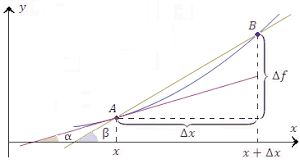
\includegraphics{img/dif.png}\\
$ AB  $ -- секущая(при $ \Delta x  \to 0$ называется касательной) \\
$ \Delta x \to 0 \Rightarrow \beta  \to \alpha  \Rightarrow \quad  \tg \beta  \to \tg \alpha  $\\
$ \tg \beta  =  \frac{\Delta y}{\Delta x}; \quad  \tg \alpha  = f'(x) $\\
$ y_k = f(x_0) + f'(x_0)(x - x_0) $ -- уравнение касательной\\
$ y_n = f(x_0) - \frac{1}{f'(x_0)} - (x - x_0) $ -- уравнение нормали \\

опр. Функция называется дифференцируемой в точку $ x_0 $  если приращение можно представить в виде $ y = A \cdot \Delta x +\alpha (\Delta x) \cdot \Delta x $,  где A незавитсамая переменная($ \Delta x \to 0 $) . 
\[
     \Delta y = A \Delta x + o(\Delta x)
   \]   
   \begin{mdframed}[backgroundcolor=blue!20] 
          Теорема 1(связь между дифференциироваемостью и существованием производной)\\
          Для того чтобу функция $ f(x) $ была дифференциируема в точке $ x_0 $ необходимо чтобы она имела производную в точке $ x_0 $ \\

          Теорема 2(связь между диф и непрерывностью)\\
          Если f(x) диф в точке  $ x_0 $  то она непрерывна в этой точке(обратное не работает)\\
       \end{mdframed}



       
2)Физическая(мгновенная и средняя скорости):\\
\[
  s = f(t) \quad v_m = \frac{f(t + \Delta t) - f(t)}{\Delta t} = \frac{\Delta f}{\Delta x}
\]
-- это скорость изменения функции.

\subsection{Основные правила дифференциирования}

\begin{align}
  \frac{d}{dx} (c) = 0, c = const\\
  \frac{d}{dx} (u \pm v) = u' \pm v'\\
  \frac{d}{dx} (uv) = u'v+u v'\\
  \frac{d}{dx} cu = c u',c=const\\
  \frac{d}{dx} \left(\frac{u}{v}\right) = \frac{u' v - uv'}{v^2}
\end{align}

\textbf{Гиперболические функции:}\\

Гиперболический синус:\\
\[
  \sh x = \frac{e^x-e^{-x}}{2}
\]
Гиперболический косинус:\\
\[
  \ch x = \frac{e^x+e^{-x}}{2}
\]
Гиперболический тангенс и котангенс:\\
\[
  \th x = \frac{\sh x}{\ch x} \quad  \cth x = \frac{1}{\th x}
\]

\subsubsection*{Понятие о частных производных}
\[
  f(x,y)
\]
\[
  f_x' = \frac{\partial f}{\partial x} \quad y=const 
\]
\[
  f_y' = \frac{\partial f}{\partial y} \quad x=const
\]

\subsection{Производная сложной функции}

\begin{align}
  \frac{d}{dx} f(u(x)) = u'(x) \cdot f'(u(x)) 
\end{align}

\subsubsection*{Производная обратной функции}

\begin{align}
  y = f(x),f'(x)\neq 0,\exists x=f^{-1}(y),\Rightarrow x_y' = \frac{1}{y_x'}
\end{align}

\subsubsection{Производная функции заданной в параметрическом виде}

\begin{align*}
  x = f(t) \quad and \quad y = g(t): x' \neq 0 \Rightarrow t = f^{-1}(x) \quad  t'_x = \frac{1}{x'_t}\\
  y = y(x) = y(x(t)) :  y'_x = y'_t  t'_x=y'_t  \frac{1}{x'_t} = \frac{y'_t}{x'_t}\\
\end{align*}


\subsubsection{Дифференциирование функции заданной неявно}

Рассмотрим неявно заданную функцию, т.е когда функця  $ y = y(x)  $ задается равенством вида $ F(x,y) = 0 $.\\
Чтобы найти производную функции заданной неявно нужно диф-вать равенство $ F(x,y) = 0 $ по переменной $ x $ при этом $ y $ считаем функцией от $ x $.\\

\[
        y'_x = \frac{\frac{\partial F}{\partial x}}{\frac{\partial F}{\partial y}} = \frac{F'_x}{F'_y}
      \]      

\subsection{Дифференциал функции}

$ \Delta f = f'(x) \Delta x + o(\Delta x) $\\

Дифференциал функции -- \[
  \Delta f = f'(x) \Delta x
\]
в дальнейшем: $ df = f'(x) dx $\\
следствие:

\[
  f'(x) = \frac{df}{dx}   
 \] 

св-ва(теже что и у производной )+ свойство инвариантности(сохранения формы):\\
1)для первого порядка: $ y(u(x)): dy = y'_x dx=y'_x u'_x dx = y'_u du $ \\
Дифференциал первого порядка функции $ y $  выражается по одной и тойже формуле независимо от того будет ли $ y $ рассматриватся как функция от независимой переменной $ x $ или от зависимой переменной $ u $.\\


\subsubsection{Применение дифференциала в приближенных вычеслениях}

При малом $ \Delta x: \quad \Delta y = dy = f'(x)\Delta x = f(x + \Delta x) - f(x) \simeq f(x) + f'(x)\Delta x $ \\

\subsection{Производные и дифференциалы высших порядков}
Производная от производной функции называется производной второго порядка:\\
\begin{align*}
   y'' = (y')' = y^{(2)}  \\
 ...\\
   y^{(n)} \\
\end{align*}


Дифференциалом второго порядка называется дифференциал от дифференциала, рассматривоемого как функция только от переменной $ x $ (при постоянном $ dx $ ):\\
\begin{align*}
       d^2y = d(dy) = d(f'(x)dx)=(f'(x)dx)'dx=f''(x) dxdx=f''(x) dx^2 \\
      ...\\
       d^ny = f^{(n)}(x) (dx)^{n} 
    \end{align*}
свойства инвариантности дифференциалы высшего порядка не обладает.\\

\subsection{Теоремы о средних значениях}

Опр.\\
$ f(x) $ достигает точки $ x = c $ локальный максимум(минимум) если существует окресность этой точки в которой выполняется: $ f(c) \geq f(x) \quad \forall x \in \cup(c)\quad (f(c) \leq f(x) \quad \forall x \in \cup(c))$, также называется экстремум(extr)\\
\newpage
\begin{mdframed}[backgroundcolor=blue!20] 
       Теорема Ферма(необходимое условие существования extr)\\
       Если $ f(x) $ имеет производную в точку $ c $ и достигает в этой точке локального эктремума то производная в этой точку равна нулю.\[
         f'(c) = 0
       \] 

       Теорема Ролля\\
       Если $ y = f(x) $ на отрезки AB, дифференцируема на этом же промежутке и значение функции на концах совпадают, то существует точка $ \xi  $ т.ч $ f'(x) = 0 $   


    \end{mdframed}

Геометрический смысл:\\
Если выполнены условия теоремы, то на графики функции существует точка $ (\xi,f(\xi))  $ касательная\\ 
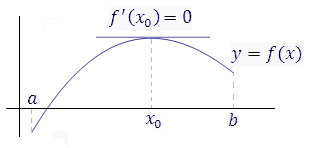
\includegraphics{img/361.png}\\

\begin{mdframed}[backgroundcolor=blue!20] 
       Теорема Коши:\\
       Если f(x),g(x) непрерывны на отрезке AB,f(x) и g(x) дифференцируемы на (a,b),g'(x) $ \neq 0 $, $ \exists \xi \in (a,b), $
       \[
           \frac{f(b)- f(a)}{g(b) - g(a)} = \frac{f'(\xi)}{g'(\xi)}
         \]  

        Теорема Лагранжа\\
        Пусть f(x) непрерывна на AB и дифференциируема на (a,b), тогда существует точка $ \xi \in (a,b): \quad f(b) = f(a) = f'(\xi)(b-a) $\\ 
    \end{mdframed}
\newpage
Геометрический смысл Т. Лагранжа:\\
\quad \quad \quad 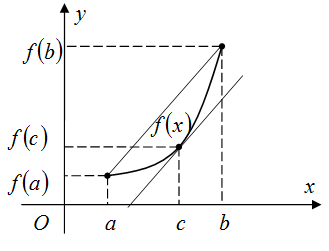
\includegraphics{img/362.png}\\
Следствие -- $ f'(x) = 0 \Rightarrow f(x) = const $ \\

\subsection{Параграф. Правила Лопиталя(раскрытие неопределенности)}
Пусть выполнены условия:\\
1)f(x),g(x) дифференциируемы в окресности точки A, за исключением ,быть может, самой точки A.\\
2)g'(x) $ \neq 0 $ в окресноти A\\
3)$ \lim_{x\to A} \frac{f(x)}{g(x)} = \left\{\frac{0}{0}\right\} \quad  or \quad \left\{\frac{inf}{inf}\right\} $\\
4)$ \exists \lim_{x\to a} \frac{f'(x)}{g'(x)} = A $\\
\[
  \Rightarrow \exists \lim_{x\to a} \frac{f(x)}{g(x)} = \lim_{x\to a} \frac{f'(x)}{g'(x)} = A
\]


Упр. $ \lim_{x\to 0} \frac{x^2 \cos(\frac{1}{x})}{\sin x} $

\newpage
\subsection{Параграф. Формула Тейлора.}
Задача: представить функцию f(x) в некоторой окресности точки A в виде многочлена относительно разности $ x - a $ (разложить по степеням).\\

Пусть f(x) имеет производную до n-ого порядка включительно,\\
Опр.
\[
    f(x) = f(a) + f'(a)(x-a) + \frac{f''(a)}{2!}(x-a)^2 + \ldots + \frac{f^{(n)}(a)}{n!}(x-a)^n + r_n(x)
  \]  

\begin{mdframed}[backgroundcolor=blue!20] 
       Локальная Теорема Тейлора\\
       Если f(x) - непрерывно-дифференцииррованна n раз в окресности A\\($ f(x),f'(x),\ldots,f^{(n)}(x) $-- непрерывно дифференциируема ),то $ r_n(x) = o((x-a)^n) $, записываем в форме Пеано.\\
    \end{mdframed}
    
Формы записи остатка по Коши и Лагранжу:\\
\begin{align*}
   r_n(x) = \frac{f^{(n+1)}(\xi)}{n!}(x-\xi)^n(x-a) \\
   r_n(x) = \frac{f^{(n+1)}(\xi)}{(n+1)}(x-a)^{n+1}\\
 \end{align*}
\textbf{Замечания(формула Маклорена)} -- если в формуле Тейлора вместо $ a $ взять нуль\\
\[
   f(x) = f(0) + f'(0)(x) + \frac{f''(0)}{2!}(x)^2 + \ldots + \frac{f^{(n)}(0)}{n!}(x)^n + r_n(x)
\] 

\subsection{Параграф. Признаки монотонности}

Опр. $ x_1 < x_2, \quad f(x) $ называется возрастающей если $ f(x_1)< f(x_2) $, неубывающая $ f(x_1) \leq f(x_2) $, убывающей $ f(x_1) > f(x_2) $, невозрастающей $ f(x_1) \geq f(x_2) $ \\
Во всех случаях функция называется монотонной(в 1 и 3 строго монотонной).\\  

\begin{mdframed}[backgroundcolor=blue!20] 
       Теорема(Признак монотонности функции)\\
       $ f(x) $- дифференцируема на AB и $ f'(x) > 0(f'(x) < 0):\forall x \in AB $, тогда $ f(x) $ возрастает(убывает) на AB.\\  
    \end{mdframed}
    
\textbf{Правило исследования на возрастание(убывание)}\\
1) находим точки в которых $ f'(x) = 0 $  или несуществует, эти точки называются критическими точками первого рода, они разбивают область определения  на интервалы монотонности\\
2) исследуем знак производной на каждом интервале\\
3) определяем, возрастает или убывает\\

\begin{mdframed}[backgroundcolor=blue!20] 
       
       Теорема(Первый достаточный признак существования экстремума)\\
       f(x) непрерывна в некоторой окресности точки $ x_0 $ и дифференциируема в каждой её точке за исключением быть может точки $ x_0 $. Если при переходе через $ x_0 $ производная меняет знак, то точки $ x_0 $ точка экстремума.\\ 

       Теорема(Второй достаточный признак существования экстремума)\\
       Пусть в окресности $ x_0 $ $ f(x) $ непрерывно дифференцируема $ (n+1) $ раз ($ f'(x_0)= f''(x_0)=\ldots =f^{(n)}(x_0)= 0 \quad f^{(n+1)}(x_0) \neq 0 $ ). Тогда если (n+1) нечетное число - в $ x_0 $ нет экстремума, четное - есть экстремум, причем если $ f^{(n+1)}(x_0) <(>) 0: x_0 - max(min)$     
    \end{mdframed}

Упр. Доказать общий случай.













\newpage
\subsection*{Литература}
Кудрявцев А.Д Курс математического анализа\\
Фихтенгольц Г.М Основы математического анализа\\
Демидович Б.П Сборник задач и упражнений по математическому анализу\\

\end{document}